\documentclass[10pt]{article}

% Lines beginning with the percent sign are comments
% This file has been commented to help you understand more about LaTeX

% DO NOT EDIT THE LINES BETWEEN THE TWO LONG HORIZONTAL LINES

%---------------------------------------------------------------------------------------------------------

% Packages add extra functionality.
\usepackage{times,graphicx,epstopdf,fancyhdr,amsfonts,amsthm,amsmath,algorithm,algorithmic,xspace,hyperref}
\usepackage[left=1in,top=1in,right=1in,bottom=1in]{geometry}
\usepackage{sect sty}	%For centering section headings
\usepackage{enumitem}
\usepackage{epsfig}
\usepackage[space]{grffile}
\usepackage{booktabs}
\usepackage{forest}
\usepackage{array}

% Some commands for changing header and footer format
\renewcommand{\headrulewidth}{0.4pt}
\renewcommand{\headwidth}{\textwidth}
\renewcommand{\footrulewidth}{0.4pt}

\setlength{\parindent}{0cm}

\newcommand{\Lab}{10}
\newcommand{\ProblemHeader}

\newcolumntype{P}[1]{>{\centering\arraybackslash}p{#1}}
\newcolumntype{M}[1]{>{\centering\arraybackslash}m{#1}}

% This will set LaTeX to look for figures in the same directory as the .tex file
\graphicspath{.} % The dot means current directory.

% Begin document
\begin{document}

% Set pagestyle
\pagestyle{fancy}

\newenvironment{Proof}[1][Proof]
  {\proof[#1]\leftskip=0.9cm\rightskip=0.9cm}
  {\endproof}

\lhead{Lab \Lab}
\rhead{\today}
\lfoot{CSCI 334: Principles of Programming Languages}
\cfoot{\thepage}
\rfoot{Spring 2024}
  
%---------------------------------------------------------------------------------------------------------
% DON'T CHANGE ANYTHING ABOVE THIS LINE
\section*{Biological Regulatory Inferential Additive Network (BRIAN) Specification}
\section*{\textit{Introduction}} 
     The human body is a carefully engineered biological system, consisting of approximately 30 trillion cells — all which must perform a diverse and dynamic set of functions to support daily living. But how do all these cells know which role to perform and successfully carry out their functions? The answer lies in biological regular networks, or BRNs, consisting of interconnected cellular components, such as genes, proteins, and metabolites, that interact through regulatory mechanisms to control the expression of genes, cellular activities, and organismal functions. \\
     
    With a single cell in humans often containing over 10,000 different types of protein, as well as each protein having a host of possible post-translational modifications, constructing a BRN becomes a graph-navigating problem which can quickly evolve to be a computational nightmare. This is where Biological Regulatory Inferential Additive Network (BRIAN) language hopes to offer improvements in the workflow of a lab scientist by automatically constructing possible biological regulatory networks from the user's input of simple existing relationships between cellular components discovered through experimental work. The language would be capable of translating this experimentally established relationship data into an adjacency matrix representation of a BRN, each row/column representing a specific component and indices representing relationships. Ultimately, the BRIAN language could use this matrix to construct a useful graphical representation of the described biological system and present possible new relationships that were gleaned after evaluation to the user. \\
    
    As a programming language, BRIAN’s strength lies in its ease of use: programs from a text file consist of a list of observed relationships between cellular components, which does not require the user to be acquainted with any level of coding. In this sense programs are extremely modular in which new experimental results can simply be appended to an already existing program. The language itself can also identify logical conflicts in the relations provided in the program through its evaluation of the adjacency matrix (described in further detail below). \\

\section*{\textit{Design Principles}} 
    On the technical side, BRIAN hopes to be a highly scalable and flexible language in the following manner:
    \begin{itemize}
    \item Since relationships between cellular components are ultimately stored in an adjacency matrix, adding new relationships between existing components has a very low storage and computational cost. Additionally, adding new components is performed by simply expanding the existing matrix. As only a single relationship between two components can exist (i.e. unknown, activates, or inhibits), a matrix of ints is sufficient to represent the BRN.

    \item BRIAN accommodates all existing proteins, genes, phenotypes (as well as an [other] category for components such as small RNAs or metabolites) and allows interactions between all these types freely. The language also does not strictly define the type of relationship between two cellular nodes: while the expected relationship types are abstract interactions (e.g. activation, inhibition), if these are not known, the biochemical modification (e.g. phosphorylation, ubiquitination, acetylation, methylation) are also accepted.

    \end{itemize}

    Aesthetically, BRIAN aims to be a clear and expressive language. Since BRIAN is a strongly-typed language, it would help users avoid confusion of variables. For example, insulin is both a protein and a gene, using BRIAN, the user can be sure which variable is under consideration at all times. However, in the user’s input this distinction can easily be made by following the common biological syntax of gene names starting with a lowercase letter and protein names with an uppercase.

\section*{\textit{Examples}}
Sample Program $\#1$:
    \\Input:
    \begin{verbatim}
    dotnet run txt/Example1.txt
        Example1.txt file:
        "Protein_A activates gene_b
        gene_b activates Protein_A
        gene_b activates Protein_C
        Protein_C inhibits Protein_D
        Protein_D inhibits Protein_D"
    \end{verbatim} 
    Output (in addition to graphical output):
    \begin{verbatim}
    Successful parse.
    New found relations: 
    Protein_A activates Protein_A
    Protein_A activates Protein_C
    Protein_A inhibits Protein_D
    gene_b activates gene_b
    gene_b inhibits Protein_D
    \end{verbatim}
    
Sample Program $\#2$:
    \\Input:
    \begin{verbatim}
    dotnet run txt/Example2.txt
        Example2.txt file:
        "gene1 inhibits Protein1
        Protein2 activates *phenotype1
        Protein2 inhibits gene3
        *phenotype2 activates gene3
        #unknown_siRNA inhibits gene4-a"
    \end{verbatim} 
    Output (in addition to graphical output):
    \begin{verbatim}
    Successful parse.
    New found relations: (None)
    \end{verbatim} 

Sample Program $\#3$:
    \\Input:
    \begin{verbatim}
    dotnet run txt/Example3.txt
        Example3.txt file:
        "A activates B
        B inhibits C
        A activates C"
    \end{verbatim} 
    Output (in addition to graphical output):
    \begin{verbatim}
    Successful parse.
    New found relations: (None)
    Contradiction Found At: A activates C
    \end{verbatim} 
    
\section*{\textit{Language Concepts}}
A typical user is expected to be familiar with cellular components, such as proteins, genes and phenotypes, which serve as primitives for BRIAN. When the user inputs a text file describing observed relationships between components, BRIAN constructs a fitting BRN and infers new relationships between the variables. In essence, BRIAN’s evaluator is designed to consider all possible combinations between the identified primitives and offer any new found ones as a result.\\

The combining forms of cellular components mainly include more abstract interactions (e.g. activation, repression), or if these are not known, the biochemical modification (e.g. phosphorylation, ubiquitination, acetylation, methylation) between two cellular components (the primitives). Upon receiving a correct file of relationship descriptions from the user, BRIAN parses and stores all relationships between cellular components in a list of relations.

\section*{\textit{Syntax}}
\begin{align*}
\langle gene \rangle ::=& \: {\langle \alpha \in \{ a ... z \} \rangle \langle \alpha \in \{ a ... z \} \cup \{ A ... Z \} \cup \{ \mathbb{Z} \} \cup \{\_,- \} \rangle}^{*} \\
\langle protein \rangle ::=& \: {\langle \alpha \in \{ A ... Z \} \rangle \langle \alpha \in \{ a ... z \} \cup \{ A ... Z \} \cup \{ \mathbb{Z} \} \cup \{\_,- \} \rangle}^{*} \\
\langle phenotype \rangle ::=& \: *{\langle \alpha \in \{ a ... z \} \cup \{ A ... Z \} \cup \{ \mathbb{Z} \} \cup \{\_,- \} \rangle}^{+} \\
\langle other \rangle ::=& \: \#{\langle \alpha \in \{ a ... z \} \cup \{ A ... Z \} \cup \{ \mathbb{Z} \} \cup \{\_,- \} \rangle}^{+} \\
\langle variable \rangle ::=& \; \langle gene \rangle \; \\
& | \; \langle protein \rangle \; \\
& | \; \langle phenotype \rangle \; \\
& | \; \langle other \rangle \\
\langle relationship \rangle ::=& 
\; \langle variable \rangle \; \mbox{activates} \; \langle variable \rangle \\
& | \; \langle variable \rangle \; \mbox{inhibits} \; \langle variable \rangle \\
\langle sequence \rangle ::=& \: {\langle relationship \rangle}^{+}
\end{align*}
\vspace{8cm}


\section*{\textit{Semantics}}

\begin{center}
\begin{tabular}{ M{4cm}|M{4cm}|M{1.5cm}|m{6cm} }
 Syntax & Abstract Syntax & Prec./Assoc. & \centering\arraybackslash Meaning \\ 
 \hline
  \verb|<gene>| & \verb|Variable| of \verb|string| & n/a  &\verb|Gene| is a primitive of type \verb|string|. \verb|Gene| is a subtype of the primary \verb|Variable| primitive and must start with a lowercase letter. \\ 
 \hline
 \verb|<protein>| & \verb|Variable| of \verb|string| & n/a  &\verb|Protein| is a primitive of type \verb|string|. \verb|Protein| is a subtype of the primary \verb|Variable| primitive and must start with a capital letter. \\ 
 \hline
 \verb|<phenotype>| & \verb|Variable| of \verb|string| & n/a  &\verb|Phenotype| is a primitive of type \verb|string|. \verb|Phenotype| is a subtype of the primary \verb|Variable| primitive and must start with a “$*$” character. \\ 
 \hline
 \verb|<other>| & \verb|Variable| of \verb|string| & n/a  &\verb|Other| is a primitive of type \verb|string|. \verb|Other| is a subtype of the primary \verb|Variable| primitive and must start with a “$\#$” character. \\ 
 \hline
  \verb|<v1>␣| activates \verb|␣<v2>| & \verb|Activation| of \verb|Variable * Variable|& n/a & \verb|Activation| indicates the relationship between two given variables, specifically \verb|v1| activates \verb|v2|. \verb|Activation| is a subtype of the primary \verb|Relation| combining form.\\ 
 \hline
 \verb|<v1>␣| inhibits \verb|␣<v2>| & \verb|Inhibition| of \verb|Variable * Variable|& n/a & \verb|Inhibition| indicates the relationship between two given variables, specifically \verb|v1| inhibits \verb|v2|. \verb|Inhibition| is a subtype of the primary \verb|Relation| combining form.\\ 
 \hline
 \verb|<Relation>|$^+$ & \verb|List| of \verb|Relation| & n/a & \verb|Sequence| contains a list of all \verb|Relations| present in a given BRN. \verb|Sequence| must take at least one \verb|Relation| to be valid.\\ 
 \hline
\end{tabular}
\end{center}

\vspace{1cm}
\textbf{About Evaluation} \\ 

Aside from the program which is contained in a .txt file, no additional input is provided. \\

To understand how evaluation works for BRIAN, let’s consider our first example. When we call
\begin{verbatim}
    eval test1.txt
\end{verbatim}
BRIAN parses the text file and classifies the cellular components into their appropriate primitive types. 

\begin{verbatim}
    Example1.txt file:
        "Protein_A activates gene_b
        gene_b activates Protein_A
        gene_b activates Protein_C
        Protein_C inhibits Protein_D
        Protein_D inhibits Protein_D"
\end{verbatim}

After parsing, BRIAN compiles a list of all unique cellular components, which in our case we have four: 
\begin{verbatim}
[Protein "Protein_A"; Gene "gene_b"; Protein "Protein_C"; Protein "Protein_D"]
\end{verbatim}

Then, a matrix (call it P) is constructed from all the parsed relationships:
$$P = \begin{pmatrix}
	0 & 1 & 0 & 0 \\
	1 & 0 & 1 & 0 \\
        0 & 0 & 0 & 2 \\
        0 & 0 & 0 & 2 \\
\end{pmatrix}$$
, where 1 signifies activation, 2 signifies inhibition and 0 means no relationship. The P matrix successfully captures the following BRN graph:

\begin{figure}[h]
    \centering
    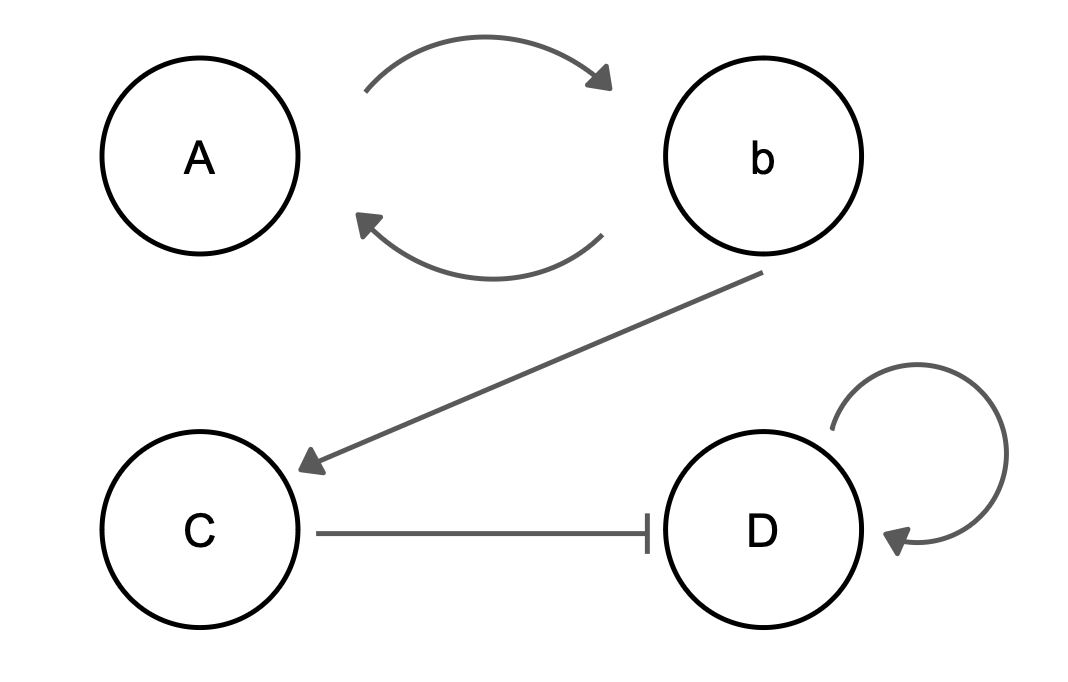
\includegraphics[width=0.5\textwidth]{BNR1}
\end{figure}

Using the P matrix, we are now ready to search for new relationships using matrix multiplication. The next step is using matrix multiplication to find new relationships. This operates under the biological logic of: 

\begin{verbatim}
    (A activates B, B activates C) implies A activates C
	        In the matrix: 1 * 1 = 1
    (A activates B, B inhibits C) implies A inhibits C
        In the matrix: 1 * 2 = 2
    (A inhibits B, B activates C) implies A inhibits C
        In the matrix: 2 * 1 = 2
    (A inhibits B, B inhibits C) implies A activates C
        In the matrix: 2 * 2 = 4, 4 is then converted to 1 (activation)
\end{verbatim}

Since the underlying relationship between cellular components does not change, we may model this traversal problem as a quasi-Markov Chain process. The transition matrix for our MC model would contain information on existing relationships, which we may probabilistically interpret as a sure event that state $i$ would go to state $j$. So, at each step (of multiplying P to itself), we capture the transfer of relationship $ij$ to relationship $jk$ in our next step, which is true to how BRN relationships function. \\

However, to avoid the summation of multiple values, each row and column of a matrix can only contain one value before being multiplied by itself. Following this logic, the following matrix derivations are made by zeroing certain values:

$$ \mbox{Matrix1} = \begin{pmatrix}
	0 & 1 & 0 & 0 \\
	1 & 0 & 0 & 0 \\
        0 & 0 & 0 & 2 \\
        0 & 0 & 0 & 0 \\
\end{pmatrix} $$

$$\mbox{Matrix2} = \begin{pmatrix}
	0 & 1 & 0 & 0 \\
	1 & 0 & 0 & 0 \\
        0 & 0 & 0 & 0 \\
        0 & 0 & 0 & 2 \\
\end{pmatrix}$$

$$\mbox{Matrix3} = \begin{pmatrix}
	0 & 1 & 0 & 0 \\
	0 & 0 & 1 & 0 \\
        0 & 0 & 0 & 2 \\
        0 & 0 & 0 & 0 \\
\end{pmatrix}$$

$$\mbox{Matrix4} = \begin{pmatrix}
	0 & 1 & 0 & 0 \\
	0 & 0 & 1 & 0 \\
        0 & 0 & 0 & 0 \\
        0 & 0 & 0 & 2 \\
\end{pmatrix}$$

And the results of multiplication:

$$\mbox{Matrix1} = \begin{pmatrix}
	1 & 0 & 0 & 0 \\
	0 & 1 & 0 & 0 \\
        0 & 0 & 0 & 0 \\
        0 & 0 & 0 & 0 \\
\end{pmatrix}$$

$$\mbox{Matrix2} = \begin{pmatrix}
	1 & 0 & 0 & 0 \\
	0 & 1 & 0 & 0 \\
        0 & 0 & 0 & 0 \\
        0 & 0 & 0 & 4 \\
\end{pmatrix}$$

$$\mbox{Matrix3} = \begin{pmatrix}
	0 & 0 & 1 & 0 \\
	0 & 0 & 0 & 2 \\
        0 & 0 & 0 & 0 \\
        0 & 0 & 0 & 0 \\
\end{pmatrix}$$

$$\mbox{Matrix4} = \begin{pmatrix}
	0 & 0 & 1 & 0 \\
	0 & 0 & 0 & 0 \\
        0 & 0 & 0 & 0 \\
        0 & 0 & 0 & 4 \\
\end{pmatrix}$$

The new values from these matrices can be added back to the original (inhibition (2) on diagonal values (representing self-inhibition) result in a 4 in the same place after squaring; in this case we do not consider this a contradiction).

$$P' = \begin{pmatrix}
	1 & 1 & 1 & 0 \\
	1 & 1 & 1 & 2 \\
        0 & 0 & 0 & 2 \\
        0 & 0 & 0 & 2 \\
\end{pmatrix}$$

From this new matrix, the following relationships are found:
 \begin{verbatim}
    New found relations: 
    Protein_A activates Protein_A
    Protein_A activates Protein_C
    gene_b activates gene_b
    gene_b inhibits Protein_D
    \end{verbatim}

Using this new graph, the same matrix derivation and multiplication process can be repeated to find new relationships, up to $log_2(n)$ times where $n$ is the number of unique elements. This results in the final matrix:
$$P' = \begin{pmatrix}
	1 & 1 & 1 & 2 \\
	1 & 1 & 1 & 2 \\
        0 & 0 & 0 & 2 \\
        0 & 0 & 0 & 2 \\
\end{pmatrix}$$

From the final matrix, the following relationships are found:
 \begin{verbatim}
    New found relations: 
    Protein_A activates Protein_A
    Protein_A activates Protein_C
    Protein_A inhibits Protein_D
    gene_b activates gene_b
    gene_b inhibits Protein_D
    \end{verbatim}

% DO NOT DELETE ANYTHING BELOW THIS LINE
%---------------------------------------------------------------------------------------------------------
\end{document}